% Base sur la VO 0.99.0
% Relecture technique: 
% Relecture syntaxique: 

\part{Règles spéciales}

Les règles spéciales sont des règles additionnelles liées à des figurines, des armes ou des sorts. Vous trouverez en détail la façon dont ces règles doivent être appliquées après la liste des règles spéciales ci-dessous.

% TODO: ajouter ici des liens vers les regles.

\subsubsection*{Attaques spéciales}

Quelques figurines possèdent des capacités inhabituelles appelées des \emph{Attaques Spéciales}, comme les \emph{Touches d'Impact} ou les \emph{Attaques de Souffle}. Ces \emph{Attaques Spéciales} n'utilisent pas l'arme de la figurine et ne bénéficient pas des règles spéciales qui modifient les attaques de corps à corps et de tir classiques (y compris des règles spéciales qui modifient des Caractéristiques). Cependant, les \emph{Attaques Spéciales} peuvent profiter d'autres types de règles (qui ne sont pas des règles spéciales) ou bénéficier d'augmentation de caractéristiques (grâce à des sorts, des objets magiques...). Par exemple, une arme lourde ou une \emph{Charge Tonitruante} ne peut pas augmenter la force des attaques de \emph{Piétinement}, mais une Potion de Force ou le sort "La Bête qui Sommeille" le peut.

Ces attaques spéciales sont:
%TODO: mettre les paragraphes en lien
\begin{itemize}
\item Attaque au passage
\item Attaque de broyage (X)
\item Attaque de souffle (X)
\item Attaque écrasante
\item Piétinement (X)
\item Touches d'impact (X) 
\end{itemize} 

\section{Liste des règles spéciales} 

\subsubsection*{Arme à deux mains}

Une figurine équipée d’une arme ayant cette règle spéciale ne peut pas utiliser simultanément de bouclier.


\subsubsection*{Attaques aléatoires (X)}

Chaque fois qu'une figurine avec cette règle spéciale doit attaquer au corps à corps, son nombre d'attaques est déterminé par le nombre entre parenthèses (X), avant d'appliquer tout modificateur. Par exemple, une figurine avec \emph{Attaques Aléatoires (1D3+2)} a un nombre aléatoire d'attaques entre 3 et 5. Ces attaques ignorent la règle qui stipule qu'une caractéristique ne peut pas dépasser 10.

\subsubsection*{Attaque au passage - Attaque Spéciale}

Attaque Spéciale \newrule{à distance}. Cette attaque peut être utilisée par les unités composées de figurines ayant cette règle. À la fin de la phase des Autres Mouvements, désignez une unité ennemie \newrule{non engagée au corps à corps} au dessus de laquelle l'unité a fait un mouvement simple ou une marche forcée pendant cette phase \newrule{(même si les socles n'ont été survolés que partiellement)}. Cette attaque peut aussi être utilisée à la fin d'une phase de magie durant laquelle l'unité a effectué un mouvement magique. L'unité entière effectue une attaque contre l'ennemi choisi. Cette attaque touche automatiquement et est résolue suivant la description dans le profil de l'unité.

\subsubsection*{\nouveau{Attaques de broyage (X)} - Attaque Spéciale}

Une figurine avec cette règle spéciale \newrule{doit} faire une \emph{Attaque Spéciale} au corps à corps à sa propre Initiative contre une unique unité ennemie en contact socle à socle avec elle. L'attaque inflige un nombre de touches automatiques égal à la valeur indiquée entre parenthèses (X), avec une Force égale à la Force de la figurine. Les \emph{Attaques de Broyage} sont des attaques spéciales et ne bénéficient jamais de l'équipement ou des règles spéciales de la figurine. Si une figurine possède à la fois des \emph{Attaques de Broyage} et des \emph{Touches d'Impact}, elle ne peut utiliser que l'une des deux dans une même \emph{Phase de Corps à Corps}. Vous pouvez choisir.

\subsubsection*{Attaque de souffle (X) - Attaque Spéciale}

Les \emph{Attaques de Souffle} peuvent être utilisées une fois par partie, soit comme une \emph{Attaque Spéciale} de tir, soit comme une \emph{Attaque Spéciale} de corps à corps. Si une figurine possède plusieurs \emph{Attaques de souffle}, elle ne peut en utiliser qu'une par phase de jeu.
\begin{itemize}[label={-}]
\item Comme une attaque spéciale de tir, normalement pendant la phase de tir: choisissez une cible en utilisant les règles normales pour les attaques de tir. \nouveau{Cette attaque a une portée de 6{\pouce}} et peut être utilisée même si la figurine a fait une \emph{Marche Forcée} ou pour Tenir la position et tirer suite à une charge.
\item Comme une attaque spéciale de corps à corps, normalement pendant la phase de corps à corps, elle est faite à l'Initiative de la figurine, ou de l'élément de la figurine qui effectue l'attaque. Déclarez que vous utilisez une \emph{Attaque de Souffle} quand vous allouez les attaques et désignez une unité en contact socle à socle à attaquer.
\end{itemize}

\nouveau{L'\emph{Attaque de Souffle}, que ce soit au corps à corps ou au tir, inflige 2D6 touches automatiques à sa cible}. La Force et les règles spéciales éventuelles de ces touches sont données entre parenthèses, comme dans \emph{Attaque de Souffle (\emph{Force 4}, Attaques Enflammées)}. Les \emph{Attaques de Souffle} sont des attaques spéciales et ne bénéficient jamais de l'équipement ou des règles spéciales de la figurine qui effectue l'attaque.

\subsubsection*{\nouveau{Attaques divines}}

Les \emph{Sauvegardes Invulnérables} réussies contre des attaques ayant cette règle spéciale, ou contre des attaques au corps à corps provenant d'une figurine ayant cette règle spéciale, doivent être relancées.

\subsubsection*{\nouveau{Attaque écrasante} - Attaque Spéciale}

Une figurine qui possède cette règle peut échanger toutes ses attaques normales de corps à corps pour effectuer une unique \emph{Attaque Spéciale}. Elle ne peut pas être effectuée en tant qu'attaque de \emph{Soutien}, est résolue à Initiative 0, avec une Force de 10 et \emph{Blessures Multiples (Artillerie)}. \newrule{L'équipement ou les règles spéciales d'une figurine ne peuvent pas améliorer son \emph{Attaque écrasante}.} La figurine peut toujours effectuer ses autres \emph{Attaques Spéciales}, comme le \emph{Piétinement} ou les \emph{Touches d'Impact}. \newrule{Même si c'est une \emph{Attaque Spéciale}, cette attaque est allouée comme si elle était une attaque normale de corps à corps.}

\subsubsection*{Attaques empoisonnées}

Lorsqu'une attaque provenant d'une figurine ayant cette règle spéciale obtient un '6' non modifié pour toucher \nouveau{(au tir comme un corps à corps)} \newrule{et si cette touche est réussie}, elle blesse automatiquement, sans qu'aucun jet pour blesser ne soit requis. Les attaques de tirs nécessitant un jet de 7+, ou plus, pour toucher ne peuvent jamais bénéficier de la règle \emph{Attaques Empoisonnées}. \newrule{Si l'attaque peut se dupliquer en plusieurs touches (comme pour un tir de baliste ou avec une arme à gabarit), une seule touche (au choix de l'attaquant) blesse automatiquement, toutes les autres doivent faire des jets pour blesser normalement.}

\subsubsection*{Attaques enflammées}

Cette règle s'applique aux attaques avec cette règle spéciale et aux attaques venant de figurines ayant cette règle spéciale, qu'elles soient de corps à corps ou de tir. Ces attaques n'ont dans un cas ordinaire aucun effet. Toutefois, elles interagissent avec d'autres règles spéciales, comme \emph{Inflammable} ou \emph{Régénération}.

\subsubsection*{\nouveau{Attaques foudroyantes}}

Les unités ayant la règle spéciale \emph{Vol} qui subissent au moins une touche avec cette règle spéciale pendant une phase reçoivent 1D6 touches de Force 4 supplémentaires à la fin de cette phase.

\subsubsection*{Attaques magiques}

Les attaques ayant cette règle spéciale ou les attaques faites par des figurines ayant cette règle spéciale n'ont dans un cas ordinaire aucun effet. Toutefois, elles interagissent avec d'autres règles spéciales, comme \emph{Éthéré}. \nouveau{Les figurines ayant cette règle spéciale l'appliquent à toutes leurs attaques, incluant les attaques spéciales comme le \emph{Piétinement}, les \emph{Touches d'Impact} et les \emph{Attaques de Souffle}}, à moins que le contraire ne soit précisé. Tous les dégâts des sorts, des fiascos et des objets magiques sont des \emph{Attaques Magiques}.

\subsubsection*{\nouveau{Attaques toxiques}}

Les attaques ayant cette règle spéciale ou les attaques de corps à corps venant de figurines ayant cette règle spéciale ont toujours Force 3 et \emph{Perforant (6)}.

\subsubsection*{Avant-garde}

Après le déploiement et après les \emph{Éclaireurs}, les unités composées entièrement de figurines ayant cette règle spéciale peuvent effectuer un mouvement de 12{\pouce}. Ce mouvement est effectué comme dans l'étape des \emph{Autres Mouvements}, avec les mêmes restrictions et actions possibles, comme faire une roue, une \emph{Reformation}, rejoindre des unités, quitter des unités, etc. La distance de 12{\pouce} est utilisée à la place de la valeur de Mouvement de la figurine et aucune \emph{Marche Forcée} n'est autorisée. Les unités faisant un mouvement d'\emph{Avant-Garde} ne peuvent pas s'approcher à moins de 12{\pouce} des unités ennemies. \newrule{Cette limite est réduite à 6{\pouce} pour une unité ennemie possédant la règle \emph{Avant-Garde} ou \emph{Éclaireur}}. Une unité faisant un mouvement d'\emph{Avant-Garde} ne peut pas déclarer de charge au premier tour si son camp commence. \nouveau{Si les deux joueurs ont des unités d'\emph{Avant-Garde}, alternez le déplacement des unités une par une, en commençant par le joueur qui a terminé son déploiement en} \newrule{dernier. Au lieu de déplacer une unité, un joueur peut déclarer ne plus déplacer d'unités ayant la règle \emph{Avant-Garde}.}

\subsubsection*{Blessures multiples (X, Y)}

Les blessures non sauvegardées causées par des attaques ayant cette règle spéciale ou des attaques de corps à corps venant de figurines avec cette règle spéciale sont multipliées par la valeur donnée entre parenthèses (X). Si la valeur est un dé, par exemple \emph{Blessures Multiples (1D3)}, lancez un dé pour chaque blessure non sauvegardée. Le nombre de blessures, une fois multiplié, ne peut jamais être plus grand que la caractéristique de PV de la cible, sans prendre en compte les blessures déjà subies précédemment dans la bataille. Par exemple, si une attaque ayant la règle \emph{Blessures Multiples (1D6)} blesse un troll, qui a 3 PVs, et obtient un \result{5} pour le nombre de blessures, elles sont réduites à 3 blessures.

\nouveau{Si (\emph{Artillerie}) est indiqué entre parenthèses, le nombre de blessures est de 1D3 + 1. Contre les cibles ayant la règle spéciale \emph{Vol}, il est augmenté à 1D3 + 2}.

\nouveau{Parfois cette règle est liée à certains types de troupe ou à des règles spéciales. Si c'est le cas, ils seront précisés entre parenthèses (Y). Par exemple, \emph{Blessures Multiples (2, Infanterie)}. Quand c'est le cas, n'utilisez la règle de \emph{Blessures Multiples} que contre les types de troupe indiqués ou contre celles possédant cette règle spéciale.}

\subsubsection*{\nouveau{Caché}}

Une figurine \emph{Cachée} peut être déployée \og cachée \fg . Si vous choisissez de faire ainsi, notez en secret dans quelle unité (non \emph{Personnage}) cette figurine est cachée au lieu de déployer la figurine. Cette unité doit déjà avoir été déployée et doit être du même type de troupe que la figurine \emph{Cachée}. De plus, la figurine doit avoir le droit de rejoindre cette unité en temps normal.

Tant qu'elle est \emph{Cachée}, une figurine ne peut ni être touchée ou affectée par quoi que ce soit, ni affecter le jeu en quoi que ce soit (par exemple attaquer, utiliser ou bénéficier d'objets magiques, ou empêcher des unités de faire leur mouvement d'\emph{Avant-garde}). À moins que l'unité qui la dissimule ne soit en fuite, la figurine peut être révélée au début de n'importe quel tour de joueur, ou au début de n'importe quelle manche de combat à laquelle l'unité participe. Placez alors la figurine à l'intérieur de l'unité comme si elle l'avait rejointe, en suivant la règle \emph{Au Premier Rang}, à l'exception près qu'elle ne peut remplacer d'autres figurines avec la règle \emph{Au Premier Rang}. Une fois révélée, la figurine agit normalement. Cette règle n'a plus d'incidence sur la partie. Si la figurine n'est jamais révélée pendant la partie, par exemple si son unité est détruite, elle compte comme détruite.

\subsubsection*{\nouveau{Camouflé}}

Les attaques de tir dirigées contre une unité dont la majorité des figurines a cette règle spéciale subissent un malus de -1 pour toucher.

\subsubsection*{Canalisation}

\nouveau{Chaque élément de figurine qui possède cette règle spéciale ajoute +1 au résultat du jet de \emph{Canalisation}. Tous les \emph{Sorciers} ont cette règle spéciale}.

\subsubsection*{Cavalerie légère}

Les figurines avec la règle spéciale \emph{Cavalerie Légère} ont également les règles spéciales \emph{Avant-Garde} et \emph{Troupes Légères}. Si une unité constituée uniquement de figurines ayant la règle \emph{Cavalerie Légère} \nouveau{déclare une fuite de façon volontaire en réaction à une charge (elle n'était donc pas déjà en fuite, et n'a pas raté de test de \emph{Terreur}), et réussit à se rallier au tour du joueur suivant, alors l'unité peut bouger normalement, comme si elle ne venait pas de se rallier}, mais elle ne peut pas charger. Elle peut aussi tirer mais compte toujours comme ayant bougé.

\subsubsection*{Charge dévastatrice}

Les figurines avec cette règle spéciale ont +1 Attaque lors du tour de joueur où elles réussissent une charge. Si une figurine en plusieurs éléments possède cette règle, alors celle-ci ne s'applique qu'aux éléments qui en disposent.

\subsubsection*{\nouveau{Charge tonitruante}}

Dans la première manche de corps à corps dans lequel elles ont chargé, les figurines avec cette règle spéciale ont +1 en Force. Ce bonus de Force ne peut être utilisé que pour les Attaques visant directement les ennemis qui viennent d'être chargés. Si une figurine en plusieurs éléments possède cette règle, alors celle-ci ne s'applique qu'aux éléments qui en disposent.

\subsubsection*{Combat avec un rang supplémentaire}

Les figurines avec cette règle spéciale peuvent effectuer des attaques de \emph{Soutien} avec un rang de plus. Ainsi, dans une formation normale, des figurines au troisième rang avec cette règle spéciale peuvent faire des attaques de \emph{Soutien}. Cette règle peut être cumulée plusieurs fois, permettant à un rang supplémentaire de faire des attaques de \emph{Soutien} pour chaque répétition.

\subsubsection*{\nouveau{Conclave de sorciers (sorts)}}

Les \emph{Champions} d'une unité ayant la règle \emph{Conclave de Sorciers} reçoivent +1 PV, en plus des augmentations de caractéristique associées aux \emph{Champions}. De plus, ce sont des \emph{Sorciers apprentis} de niveau 1. Le \emph{Champion} connaît des sorts prédéterminés, qui sont définis entre parenthèses. Par exemple, un champion d'un \emph{Conclave de Sorciers (niveau 1 : Feu d'Azur, Bûcher Carmin)} sera un \emph{Sorcier apprenti} de niveau 1 avec deux sorts prédéterminés, Feu d'Azur et Bûcher Carmin.

\subsubsection*{Coup fatal}

Si une attaque ayant cette règle spéciale, ou une attaque de corps à corps provenant d'une figurine ayant cette règle spéciale obtient \nouveau{un résultat non modifié de \result{6} pour blesser, cette blessure suit la règle \emph{Perforant (6)} et aucune \emph{Régénération} ne peut être utilisée contre elle}. Si une figurine en plusieurs éléments possède cette règle, alors celle-ci ne s'applique qu'aux éléments qui en disposent.

\subsubsection*{\nouveau{Distrayant}}

Les attaques de corps à corps dirigées vers une figurine qui possède cette règle spéciale subissent un malus de -1 pour toucher. Ce modificateur ne peut pas être combiné avec un autre malus pour toucher au corps à corps, comme un autre -1 pour toucher.

\subsubsection*{\nouveau{D'Outre-Monde}}

Les figurines avec cette règle spéciale font des \emph{Attaques Magiques}, sont \emph{Immunisées à la Psychologie} et ont une \emph{Sauvegarde Invulnérable (5+)}. Les \emph{Personnages} ayant la règle spéciale \emph{D'Outre-Monde} sont les seuls à pouvoir rejoindre une unité \emph{D'Outre-Monde} et ne peuvent rejoindre que des unités \emph{D'Outre-Monde}.

\subsubsection*{Éclaireurs}

\nouveau{Avant de déployer une armée qui inclut des unités ayant la règle spéciale \emph{Éclaireurs}, vous devez décider quelles seront les unités déployées en \emph{Éclaireurs} (en commençant par le joueur qui a choisi sa zone de déploiement). Déployez ensuite votre armée normalement à l'exception des unités déployées en \emph{Éclaireurs}. Les \emph{Éclaireurs} sont déployés une fois que toutes les autres unités ont été déployées}. Vous pouvez alors soit les déployer dans votre zone de déploiement, en suivant les règles normales, soit les déployer en dehors de votre zone de déploiement, mais à \nouveau{plus de 18{\pouce} de toute unité ennemie}. \newrule{Cette limite est abaissée à 12{\pouce} si l'unité d'\emph{Éclaireurs} est entièrement déployée dans une Forêt, une Ruine, un Bâtiment, un Champ ou une Eau peu profonde.} Les \emph{Éclaireurs} déployés en dehors de leur zone de déploiement ne peuvent pas déclarer de charge lors du premier tour si leur camp a eu le premier tour. Si les deux joueurs ont des \emph{Éclaireurs}, alternez le déploiement de ces unités, une par une, en commençant par celui qui a fini de se déployer en premier.

\subsubsection*{Embuscade}

\nouveau{Avant de déployer une armée qui inclut des unités ayant la règle spéciale \emph{Embuscade} (mais après avoir déterminé les zones de déploiement), vous devez décider quelles seront les unités déployées en \emph{Embuscade} (en commençant par le joueur qui a choisi sa zone de déploiement). Déployez ensuite votre armée normalement à l'exception des unités embusquées, qui ne doivent pas être déployées.} À partir du deuxième tour, lancez un dé au début de chacune de vos étapes \emph{Autres Mouvements} pour chaque unité en \emph{Embuscade}. Sur un résultat de 3+, l'unité embusquée entre sur le champ de bataille par n'importe quel bord de table. Placez l'unité avec son rang arrière au contact du bord de table. L'unité peut bouger librement pendant l'étape des \emph{Autres Mouvements}, excepté qu'elle ne peut pas effectuer de \emph{Marche Forcée} et doit finir son déplacement à une distance inférieure au double de sa valeur de mouvement (en pouces) du bord de table. Si une unité embusquée n'obtient jamais le résultat de 3+ nécessaire pour entrer sur le champ de bataille avant la fin de la partie, elle est comptée dans les pertes. \nouveau{Un personnage en \emph{Embuscade} peut être déployé avec une unité en  \emph{Embuscade} qu'il peut normalement rejoindre (précisez-le quand vous déclarez quelles unités sont en \emph{Embuscade}). Dans ce cas, effectuer un seul jet de dé pour les deux.} Jusqu'à son arrivée sur le champ de bataille, une unité en \emph{Embuscade} ne peut ni être la cible d'effet, ni faire d'action. Aucun objet magique, règle ou capacité ne peut être utilisé tant que l'unité n'est pas sur le champ de bataille.

\subsubsection*{\nouveau{Encombrant}}

Un tir provenant d'une arme avec cette règle spéciale souffre d'un malus additionnel de -1 (pour un total de -2) pour tirer après avoir bougé. Si la règle \emph{Tir rapide} s'applique aussi à ce tir, ignorez uniquement le -1 pour toucher normal dû au mouvement, pas celui lié à la règle \emph{Encombrant}.

\subsubsection*{Éthéré}

Les figurines avec cette règle spéciale font des \emph{Attaques Magiques} et ont une \nouveau{\emph{Sauvegarde Invulnérable (2+)}} qui ne peut pas être utilisée contre des \emph{Attaques Magiques}. Les \emph{Personnages} ne peuvent pas rejoindre des unités qui contiennent des figurines ordinaires \emph{Éthérées}, à moins qu'ils ne le soient eux-mêmes. De plus, les figurines avec cette règle spéciale traitent tous les terrains et décors comme du \emph{Terrain Découvert} pour tout mouvement, mais ne peuvent finir leur mouvement sur ou à moins de 1{\pouce} d'un \emph{Terrain Infranchissable}.

Si une figurine en plusieurs éléments possède cette règle, les montures ne bénéficient que des \emph{Attaques Magiques} et du mouvement facilité en traitant tout terrain comme du \emph{Terrain Découvert}. Elles ne bénéficient donc pas de la \emph{Sauvegarde Invulnérable} et ne peuvent rejoindre d'unité \emph{Éthérée} à moins que le cavalier le soit lui-même.

\subsubsection*{\nouveau{Flammes de l'Enfer}}

Toute unité subissant une ou plusieurs blessures non sauvegardées provenant d'une figurine ou d'une attaque avec cette règle spéciale pendant une phase subit 1D3 touches additionnelles de Force 3.

\subsubsection*{Frénésie}

Les figurines avec la règle spéciale \emph{Frénésie} ont +1 Attaque et sont \emph{Immunisés à la Psychologie}. Après que toutes les charges aient été déclarées, chaque unité contenant au moins une figurine ou élément de figurine ayant la \emph{Frénésie} et n'ayant pas déclaré de charge doit faire un test de Commandement. S'il est raté, l'unité doit déclarer une charge contre l'unité ennemie la plus proche pouvant être chargée, s'il y en a une. Un \emph{Personnage} ne peut cependant jamais être forcé à charger en dehors d'une unité. De plus, les unités contenant des \emph{Frénétiques} doivent toujours poursuivre ou faire une \emph{Charge Irrésistible} quand elles en ont l'occasion. Si un élément de figurine \emph{Frénétique} perd un corps à corps, il perd immédiatement la \emph{Frénésie}. Si une figurine en plusieurs éléments possède cette règle, alors celle-ci ne s'applique qu'aux éléments qui en disposent.

\subsubsection*{Fusion du métal}

Les attaques ayant cette règle spéciale ou les attaques de corps à corps faites par des figurines ayant cette règle spéciale ne demandent pas des jets pour blesser normaux. Le résultat de leurs jets pour blesser doit être supérieur ou égal à la sauvegarde d'armure de la cible. \nouveau{Un \result{6} non modifié est toujours une réussite} et un \result{1} non modifié est toujours un échec. Ces attaques ont les règles spéciales \emph{Perforant (6)} et \emph{Attaques Enflammées}. Si une figurine en plusieurs éléments possède cette règle, alors celle-ci ne s'applique qu'aux éléments qui en disposent.

\subsubsection*{\nouveau{Garde du corps (X)}}

Un \emph{Personnage} qui rejoint une unité qui contient au moins la moitié de figurines avec cette règle spéciale gagne la règle spéciale \emph{Tenace}. Quelquefois, ce bonus n'est autorisé qu'avec certains \emph{Personnages}. Quand c'est le cas, les \emph{Personnages} en question seront indiqués entre parenthèses (X).

\subsubsection*{Grande cible}

\nouveau{Une \emph{Grande Cible} ne peut jamais être rejointe ou rejoindre une unité, à moins que cette \emph{Grande Cible} soit une \emph{Plateforme de Guerre}}. Une \emph{Grande Cible} augmente la portée des règles \emph{Tenez les Rangs} et \emph{Présence Charismatique} de 6{\pouce}. Notez que la règle \emph{Grande Cible} affecte également la taille de la figurine.

\subsubsection*{Guide}

Les figurines ayant cette règle spéciale réussissent automatiquement les tests de terrain dangereux causés par les terrains et décors. Elle ne peuvent pas être empêchées d'effectuer une marche forcée à cause d'un terrain ou décor. De plus, \nouveau{elles ne perdent jamais leur règle \emph{Indomptable} ou leurs bonus de rangs à cause des terrains et décors}. Quelquefois, cette règle spéciale est uniquement associée à un terrain ou décor spécifique, indiqué entre parenthèse. Quand c'est le cas, la règle \emph{Guide} s'applique uniquement pour le type de décor ou terrain spécifié.

\subsubsection*{Haine}

Les figurines ayant cette règle spéciale peuvent relancer les jets pour toucher ratés durant la première manche d'un corps à corps. Quelquefois, la \emph{Haine} ne s'applique que contre certains ennemis, qui sont alors indiqués entre parenthèses. Par exemple, \emph{Haine (Livre d'armée : L'Empire de Sonnstahl)} veut dire que la haine s'applique quand on attaque des figurines provenant du livre d'armée de L'Empire de Sonnstahl. Si une figurine en plusieurs éléments possède cette règle, alors celle-ci ne s'applique qu'aux éléments qui en disposent.

\subsubsection*{Immunisé à la psychologie}

Si la moitié au moins des figurines d'une unité est \emph{Immunisée à la Psychologie}, l'unité réussit automatiquement tout test de \emph{Panique}, et ne peut pas déclarer de réaction de fuite à une charge, à moins qu'elle soit déjà en fuite. Les figurines \emph{Immunisées à la Psychologie} sont immunisées aux effets de la \emph{Peur}.

\subsubsection*{Indémoralisable}

Les unités \emph{Indémoralisables} réussissent automatiquement tout test de \emph{Moral}. De plus, les figurines ayant cette règle spéciale sont aussi \emph{Immunisées à la Psychologie}. Les \emph{Personnages} \emph{Indémoralisables} ne peuvent rejoindre que des unités \emph{Indémoralisables}. Les unités \emph{Indémoralisables} ne peuvent être rejointes que par des \emph{Personnages} \emph{Indémoralisables}.

\subsubsection*{Inflammable}

Les attaques ayant la règle spéciale \emph{Attaques Enflammées} \nouveau{doivent relancer leurs jets pour blesser ratés} contre les figurines étant \emph{Inflammables}. Les unités en garnison dans un bâtiment sont toujours \emph{Inflammables}.

\subsubsection*{\nouveau{Ingénieur}}

Une figurine avec cette règle spéciale permet à une \emph{Machine de Guerre} dans un rayon de 3{\pouce} d'utiliser la CT de l'\emph{Ingénieur} à la place de la sienne et de relancer n'importe quel résultat obtenu sur le tableau des incidents de tir. S'il y a plusieurs \emph{Machines de Guerre} à portée de 3{\pouce}, déclarez quelle machine recevra l'aide de l'ingénieur avant de la faire tirer. De plus, si une \emph{Machine de Guerre} possède une arme d'artillerie parmi un des types ci-dessous, l'\emph{Ingénieur} apporte un bonus additionnel et la machine pourra relancer :
\begin{itemize} [label={-}]
\item \emph{Catapulte}, le dé de déviation.
\item \emph{Canon à flamme}, le D6 pour la distance de mouvement du gabarit, à moins que le résultat ne soit \result{6}.
\end{itemize}
Une figurine engagée dans un corps à corps ne peut pas utiliser ces règles.

\subsubsection*{\nouveau{Insignifiant}}

Les unités composées entièrement de figurines ayant cette règle spéciale ne causent pas de tests de \emph{Panique} aux unités n'étant pas \emph{Insignifiantes}. Seuls des \emph{Personnages} \emph{Insignifiants} peuvent rejoindre des unités avec des figurines ordinaires \emph{Insignifiantes}.

\subsubsection*{Instable}

Les unités \emph{Instables} réussissent automatiquement tout test de \emph{Moral}. Quand une unité avec cette règle spéciale perd un combat, elle subit autant de blessures que le résultat du combat qu'elle a perdu, sans aucune sauvegarde autorisée.

Le nombre de blessures subies est réduit dans certaines situations. Appliquez les modificateurs suivants dans cet ordre:
\begin{enumerate}
\item \nouveau{Si l'unité est \emph{Tenace}, divisez par 2 le nombre de blessures subies (en arrondissant au supérieur).}
\item \nouveau{Si l'unité est \emph{Indomptable}, réduisez le nombre de blessures subies à 12 s'il est supérieur.}
\item \nouveau{Si l'unité bénéficie de la règle \emph{Tenez vos rangs!} (c'est-à-dire qu'elle est proche du \emph{Porteur de la Grande Bannière}), déduisez le \emph{Bonus de rangs} de l'unité au nombre de blessures subies. Les unités n'ayant pas de \emph{Bonus de rangs} déduisent 1 au nombre de blessures subies à la place.}
\end{enumerate}
Appliquez tout autre modificateur (objet magique, règle spéciale, sort, etc) après ces trois étapes.

Les blessures sont distribuées dans cet ordre :
\begin{enumerate}
\item Figurines ordinaires.
\item \emph{Champion}.
\item Autres \emph{Personnages}, distribuées par le joueur à qui appartient l'unité.
\end{enumerate}

\subsubsection*{Instabilité Démoniaque}

Les unités possédant cette règle ne fuient jamais au combat. À la place, le joueur doit lancer 2D6 comme pour un test de moral normal, ajouter la différence de \emph{Résultat de Combat}, puis retrancher la valeur de Commandement de l'unité. Formule simplifiée: $\textbf{2D6 + RC - Cd}$. Ce test est raté si le total est un nombre positif: l'unité subit alors un nombre de blessures égal à ce nombre. Ces blessures sont distribuées comme pour la règle \emph{Instable}, sans aucune sauvegarde autorisée. Si une unité possède les règles \emph{Instable} et \emph{Instabilité Démoniaque}, ignorez \emph{Instable} et utilisez ces règles à la place.

\subsubsection*{\nouveau{Maîtres d'armes}}

Au début de chaque manche de corps à corps, une figurine étant \emph{Maître d'Armes} peut choisir avec quelle arme elle va combattre. Cela permet notamment de choisir son Arme de base même si elle a d'autres armes. Si la figurine possède une Arme magique, elle doit par contre l'utiliser. Si une figurine en plusieurs éléments possède cette règle, alors celle-ci ne s'applique qu'aux éléments qui en disposent.

\subsubsection*{Maître de la Discipline (X)}

Les \emph{Sorciers} ayant cette règle spéciale ne déterminent pas leurs sorts aléatoirement comme d'habitude, mais peuvent à la place \nouveau{choisir librement leurs sorts} dans la \emph{Discipline} indiquée entre parenthèses (X). Ils ne peuvent toujours pas dupliquer de sort autre que le sort \emph{Primaire}.

\subsubsection*{Mort-vivant}

Les unités ayant cette règle spéciale sont \emph{Instables} et \emph{Immunisées à la Psychologie}. Elles ne peuvent pas effectuer de \emph{Marche Forcée} à moins de commencer leur mouvement \nouveau{à portée de la \emph{Présence Charismatique} du \emph{Général}}. La seule réaction de charge qu'une unité avec la règle \emph{Mort-Vivant} peut déclarer est \emph{Tenir la Position}.

\subsubsection*{Mouvement aléatoire (X)}

Les unités avec cette règle spéciale ne peuvent pas déclarer de charge ou bouger pendant l'étape des \emph{Autres Mouvements}. À la place, elles bougent lors de l'étape des \emph{Mouvements Obligatoires} en utilisant les règles suivantes. Les figurines ayant cette règle spéciale chargent, fuient, poursuivent et font des \emph{Charges Irrésistibles} sur la distance indiquée entre parenthèses (X). Elles ne peuvent jamais bénéficier de la règle \emph{Rapide}.

\nouveau{Durant l'étape des \emph{Mouvement Obligatoires}, les unités avec cette règle spéciale bougent en utilisant toutes les règles de \emph{Poursuite}, excepté qu'elles peuvent choisir librement vers quelle direction s'orienter avant de jeter les dés pour la distance de poursuite, et ne peuvent pas sortir du champ de bataille}. \nouveau{De plus, elles ne font des tests de \emph{Terrain Dangereux} que lorsqu'elles chargent un ennemi (elles continuent de tester normalement lors d'un mouvement de \emph{Fuite}, de \emph{Poursuite} ou de \emph{Charge Irrésistible}).}

Si une unité avec cette règle spéciale est en garnison dans un bâtiment, elle doit le quitter en se plaçant à 1{\pouce} du bâtiment (ou aussi proche que possible), durant l'étape des \emph{Mouvements Obligatoires}, puis être déplacée suivant les règles normales de \emph{Mouvement Aléatoire}. Elle ne peut cependant pas charger à ce même tour, et s'arrête à 1{\pouce} de tout ennemi à la place. Les \emph{Personnages} avec \emph{Mouvement Aléatoire} ne peuvent rejoindre que des unités avec la même règle spéciale. Pour ce faire, ils doivent se déplacer jusqu'à être en contact avec cette unité pendant l'étape des \emph{Mouvements Obligatoires}. Les unités ayant cette règle spéciale ne peuvent être rejointes que par des \emph{Personnages} ayant un \emph{Mouvement Aléatoire} aussi. Si une unité a plusieurs valeurs de \emph{Mouvement Aléatoire}, utilisez la plus basse disponible.

\subsubsection*{Mouvement ou tir}

Les armes de tir et les figurines ayant cette règle spéciale ne peuvent pas tirer si elles ont effectué un mouvement à ce tour de joueur. Si une figurine en plusieurs éléments possède cette règle, alors celle-ci ne s'applique qu'aux éléments qui en disposent.

\subsubsection*{\nouveau{Né du feu}}

Les figurines ayant cette règle spéciale ont une \emph{Sauvegarde Invulnérable (2+)} contre les \emph{Attaques Enflammées}. Si une figurine en plusieurs éléments possède cette règle, alors celle-ci ne s'applique qu'aux éléments qui en disposent.

\subsubsection*{Pas de marche forcée}

Les unités comprenant au moins une figurine avec cette règle ne peuvent pas effectuer de \emph{Marche Forcée}.


\subsubsection*{\nouveau{Pas un meneur}}

Les figurines ayant cette règle spéciale ne peuvent jamais être le \emph{Général} de l'armée.

\subsubsection*{Perforant (X)}

Les attaques de corps à corps faites par des figurines avec cette règle spéciale imposent un malus de \nouveau{–X à la sauvegarde d'armure} de l'ennemi en plus du malus venant de la Force de l'attaque, X étant le nombre entre parenthèses (X). Quand une arme, un sort ou une attaque spéciale possède cette règle, la règle s'applique uniquement aux attaques causées par cette arme, ce sort ou cette attaque spéciale. Si une figurine a plusieurs fois la règle spéciale \emph{Perforant} avec plusieurs valeurs, n'additionnez pas les valeurs ensemble, utilisez simplement la valeur la plus haute disponible. Si une figurine en plusieurs éléments possède cette règle, alors celle-ci ne s'applique qu'aux éléments qui en disposent.

\nouveau{Si la valeur entre parenthèses est précédée d'un signe $+$, ajoutez cette valeur à toute règle \emph{Perforant} déjà possédée par la figurine. Si la figurine ne possède pas encore cette règle, appliquer directement la valeur indiquée.}

\subsubsection*{Peur}

\nouveau{Toutes les unités ennemies en contact socle à socle avec une ou plusieurs figurines causant la \emph{Peur} souffrent d'un modificateur de -1 à leur Commandement. Les figurines étant \emph{Immunisées à la Psychologie} ou causant elles-mêmes la \emph{Peur} sont immunisées aux effets de la \emph{Peur}}. Au début de chaque manche de corps à corps, les unités en contact socle à socle avec une ou plusieurs figurines ennemies causant la \emph{Peur} doivent effectuer un test de Commandement. Si le test échoue, les figurines dans l'unité voient leur Capacité de Combat réduite à 1 pour le reste de la \emph{Phase de Corps à Corps}.

\subsubsection*{Piétinement \nouveau{(X)}}

Une figurine avec cette règle spéciale doit faire une \emph{Attaque Spéciale} de corps à corps, à Initiative 0, contre une seule unité ennemie au contact socle à socle, et ce uniquement si l'unité cible est de type \emph{Infanterie}, \emph{Bête de guerre}, \emph{Nuée} ou \nouveau{\emph{Machine de guerre}}. Cette attaque inflige un nombre de touches automatiques égal à la valeur indiquée entre parenthèses (X). Elles sont faites avec une Force égale à celle de la figurine. \newrule{Une attaque de \emph{Piétinement} ne peut jamais être allouée à une figurine n'étant pas du type cité plus haut. Les \emph{Piétinements}, étant des attaques spéciales, ne bénéficient jamais de l'équipement et des règles spéciales de la figurine. \nouveau{Si une figurine en plusieurs éléments possède cette règle, alors celle-ci ne peut être utilisée que par la monture.}}

\subsubsection*{\nouveau{Plateforme de guerre}}

Les figurines ayant cette règle spéciale peuvent rejoindre les unités comme si elles étaient des \emph{Personnages}, même si elles ne sont pas des \emph{Personnages} et même si elles sont des \emph{Grandes Cibles}. Ces figurines suivent les règles des \emph{Personnages} en ce qui concerne la répartition des touches. Quand elles rejoignent une unité avec 5 figurines ou plus (sans compter la \emph{Plateforme de Guerre}), elles peuvent participer à une \emph{Marche Forcée} même si leur type de troupe leur interdit normalement, pour des \emph{Chars} par exemple. Quand elles rejoignent une unité, elles doivent toujours être placées au centre du premier rang, éventuellement en repoussant derrière des figurines ayant la règle \emph{Au Premier Rang} \newrule{et doivent toujours garder cette position centrale}. Si la figurine ne peut pas être placée au centre du premier rang, à cause de socles non compatibles ou si l'unité est trop étroite, la \emph{Plateforme de Guerre} ne peut pas rejoindre l'unité. Cela signifie que la \emph{Plateforme de Guerre} ne peut jamais rejoindre une unité avec des socles incompatibles et qu'il ne peut y avoir qu'une seule \emph{Plateforme de Guerre} par unité. Les figurines possédant cette règle spéciale perdent la règle spéciale \emph{Rapide}.

\subsubsection*{Rapide}

Quand une unité composée entièrement de figurines ayant cette règle spéciale doit lancer les dés pour la distance de charge, fuite ou poursuite, elle lance un dé de plus, atteignant normalement 3D6, et défausse le dé avec le résultat le plus bas.

\subsubsection*{\nouveau{Rechargez!}}

Une arme de tir ou figurine avec la règle \emph{Rechargez!} ne peut jamais choisir de réagir à une charge par \emph{Tenir sa Position et Tirer}. Si une figurine en plusieurs éléments possède cette règle, alors celle-ci ne s'applique qu'aux éléments qui en disposent.

\subsubsection*{\nouveau{Réflexes foudroyants}}

Les figurines avec des \emph{Réflexes Foudroyants} ont un bonus de +1 pour toucher lors de leurs attaques de corps à corps. Cela ne s'applique pas si les figurines attaquent à Initiative 0, par exemple avec des Armes lourdes ou sous l'effet de certains sorts. Dans un tel cas, elles frappent à leur propre Initiative, au lieu d'être reléguées à une Initiative 0. Si une figurine en plusieurs éléments possède cette règle, alors celle-ci ne s'applique qu'aux éléments qui en disposent.

\subsubsection*{Régénération (X)}

La \emph{Régénération} est une sauvegarde spéciale, qui est effectuée après les jets ratés de sauvegarde d'armure. La valeur de la sauvegarde est indiquée entre parenthèses (X). Les sauvegardes de \emph{Régénération} ne peuvent pas être effectuées après une \emph{Sauvegarde Invulnérable}. Si une figurine possède les deux, choisissez laquelle utiliser. La \emph{Régénération} ne peut pas être utilisée contre des \emph{Attaques Enflammées} \nouveau{ou des \emph{Coups Fatals} ayant obtenu un \result{6} pour blesser.}

\subsubsection*{Résistance à la Magie (X)}

Toutes les figurines d'une unité avec au moins une figurine ayant la règle \emph{Résistance à la Magie} ajoutent la valeur entre parenthèses (X) à leurs jets de \emph{Sauvegarde Invulnérable}, en utilisant les mêmes règles que les sauvegardes d'armure, mais uniquement contre des blessures causées par des effets de sorts. Rappelez-vous que la \emph{Résistance à la Magie}, comme la plupart des règles spéciales, ne se cumule pas.

\subsubsection*{Sauvegarde invulnérable (X)}

Les \emph{Sauvegardes Invulnérables} sont des sauvegardes spéciales, tentées après les sauvegardes d'armure ratées. La valeur de la sauvegarde est indiquée entre parenthèses (X). Les \emph{Sauvegardes Invulnérables} ne peuvent pas être faites en plus de sauvegardes de \emph{Régénération}. Si une figurine possède les deux, choisissez laquelle utiliser.

\subsubsection*{Stupide}

Au début de votre tour, chacune de vos unités avec au moins une figurine ou élément de figurine \emph{Stupide} doit passer un test de Commandement si elle n'est pas en fuite ou engagée au corps à corps. Si le test est raté, l'unité doit bouger de 1D6{\pouce} tout droit, en s'arrêtant à 1{\pouce} des \emph{Terrains Infranchissables} et des autres unités, à l'étape des \emph{Mouvements Obligatoires}. Elle ne peut alors effectuer aucune autre action volontaire à ce tour de joueur, comme charger, bouger, tirer, lancer des sorts, etc. Si la figurine n'a pas de front, par exemple si son socle est rond, elle se déplace dans une direction aléatoire. Toutes les figurines ayant la règle spéciale \emph{Stupide} sont également \emph{Immunisées à la Psychologie}.

\subsubsection*{Tenace}

Une unité qui contient au moins une figurine \emph{Tenace} ignore toutes les pénalités dues au \emph{Résultat de Combat} sur son Commandement quand elle effectue des tests de \emph{Moral} ou des tests de \emph{Reformation de Combat}.

\subsubsection*{Terreur}

Quand une unité avec au moins une figurine causant la \emph{Terreur} déclare une charge, la cible doit faire un test de \emph{Panique}. Si le test est raté, la cible de la charge doit déclarer une réaction de fuite, si elle est autorisée à le faire. De plus, toutes les figurines causant la \emph{Terreur} causent aussi la \emph{Peur}, et sont immunisées à la \emph{Peur} et la \emph{Terreur}.

\subsubsection*{Tir de volée}

\nouveau{Un tir avec cette règle spéciale ignore les figurines faisant obstacle en terme de couvert quand elle tire. Il n'ignore pas les décors, et il doit toujours y avoir une ligne de vision sur la cible.}

\nouveau{De plus, quand elles n'effectuent pas un tir de réaction à une charge, et si l'unité n'a pas bougé lors de sa dernière phase de mouvement, toutes les figurines avec la règle \emph{Tir de Volée} peuvent tirer, même si elles sont plus loin que les deux premiers rangs normalement autorisés à tirer}. Si une figurine en plusieurs éléments possède cette règle, alors celle-ci ne s'applique qu'aux éléments qui en disposent.

\subsubsection*{Tirs multiples (X)}

Les armes de tir et les figurines ayant cette règle spéciale peuvent choisir de tirer plusieurs fois à la place d'une seule fois, à chaque phase de tir. Le nombre de tirs possibles est précisé entre parenthèses (X). Utiliser cette règle spéciale inflige un malus de -1 pour toucher pour tous les tirs effectués. Si une figurine ordinaire dans une unité utilise la règle \emph{Tirs Multiples}, les autres figurines ordinaires doivent faire de même. Si une figurine en plusieurs éléments possède cette règle, alors celle-ci ne s'applique qu'aux éléments qui en disposent.

\subsubsection*{Tir rapide}

Les tirs provenant de sources avec cette règle spéciale n'ont pas le malus de -1 pour tirer après un mouvement et peuvent toujours permettre la réaction à une charge \emph{Tenir la Position et Tirer}, quelque soit la distance à laquelle se situe l'unité chargeant. Si une figurine en plusieurs éléments possède cette règle, alors celle-ci ne s'applique qu'aux éléments qui en disposent.

\subsubsection*{Tirailleurs}

Les figurines de \emph{Tirailleurs} ont également la règle spéciale \nouveau{\emph{Troupes Légères}}. Tirer sur des \emph{Tirailleurs} se fait avec un malus supplémentaire de -1 pour toucher.

Les \emph{Tirailleurs} ne sont pas placés en contact socle à socle les uns avec les autres, mais les figurines sont espacées \nouveau{de 0,5{\pouce}}. À part cet intervalle entre les figurines, ils suivent les règles normales de formation d'unités : ils ont un front, des flancs, etc. \nouveau{Une unité de \emph{Tirailleurs} ne peut être rejointe que par des Personnages qui ont le même type de troupes que l'unité.} Quand il rejoint une unité de \emph{Tirailleurs}, un Personnage devient \emph{Tirailleur} aussi longtemps qu'il reste dans l'unité et, à moins qu'il n'ait exactement la même taille de socle que les autres figurines de l'unité, il est toujours considéré comme ayant un \emph{Socle Incompatible}. Notez que lorsque toutes les figurines d'une unité possédant la règle \emph{Tirailleurs} sont tuées, l'unité perd la règle immédiatement: contractez l'unité pour lui donner une formation normale.

Si une unité de \emph{Tirailleurs} déclare une charge ou une réaction à une charge autre que la fuite, elle est immédiatement rassemblée pour aboutir à une formation classique (voir figure \ref{figure/tirailleurs}). \nouveau{Lors de cette contraction, la figurine la plus proche de l'unité chargée ou en charge ne doit pas bouger}. Si plusieurs figurines sont éligibles (parce qu'elles sont à la même distance), le joueur actif choisit la figurine qui est considérée comme la plus proche. Les \emph{Tirailleurs} regagnent leur formation étendue s'ils ne sont plus engagés au corps à corps au début d'une \emph{Phase de Mouvement} (de tout joueur). Gardez alors le centre du premier rang immobile. S'il n'y a pas assez d'espace pour que l'unité regagne sa formation étendue, gardez l'unité en formation serrée jusqu'au premier instant où il y a assez de place.

\begin{figure}[!htbp]
\centering
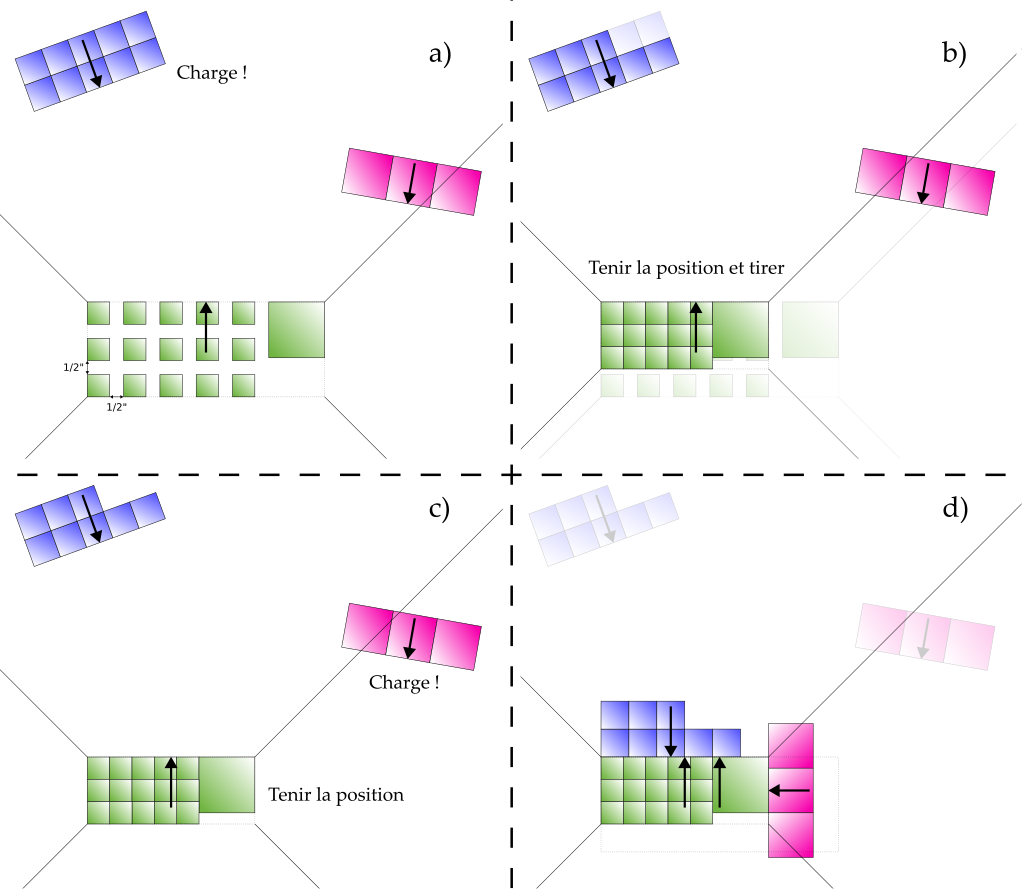
\includegraphics[width=15.5cm]{tirailleurs.png}
\caption{L'unité verte est une unité de \emph{Tirailleurs}, rejointe par un \emph{Personnage} avec un socle incompatible. \\
a) L'unité bleue lui déclare une charge. \\
b) L'unité verte déclare qu'elle va \emph{Tenir sa Position et Tirer}. Elle est immédiatement contractée. Elle fait deux victimes au tir dans l'unité bleue. \\
c) L'unité rose déclare maintenant une charge. Remarquez qu'elle est désormais dans l'arc latéral de l'unité verte. \\
d) L'unité verte déclare qu'elle va \emph{Tenir sa Position}. Les unités sont déplacées au contact.}
\label{figure/tirailleurs}
\end{figure}

\subsubsection*{Touches d'impact (X) - Attaques Spéciales}

Les \emph{Touches d'Impact} sont des \emph{Attaques Spéciales} de corps à corps qui ne doivent être utilisées que lors d'une phase de corps à corps suivant une phase
où la figurine a réussi une charge. Elles sont résolues à \nouveau{Initiative 10} contre une unique unité en contact socle à socle. Cette attaque inflige un nombre de touches automatiques égal à la valeur indiquée entre parenthèses (X), avec une Force égale celle de la figurine \nouveau{et un bonus de +1 à la Force pour chaque rang complet après le premier, à condition que l'unité soit uniquement constituée de figurines avec la règle spéciale \emph{Touches d'Impact}.} Les \emph{Touches d'Impact}, étant des attaques spéciales, ne peuvent jamais bénéficier d'un équipement ou d'une règle spéciale de la figurine influençant les attaques normales. \nouveau{Si une figurine possède à la fois des \emph{Attaques de Broyage} et des \emph{Touches d'Impact}, elle ne peut utiliser que l'une des deux au choix dans une même \emph{Phase de Corps à Corps} (vous êtes libres de choisir celle que vous souhaitez utiliser).}

\nouveau{Si la valeur entre parenthèses est précédée d'un signe $+$, ajoutez cette valeur à toute règle \emph{Touches d'Impact} déjà possédée par la figurine. Si la figurine ne possède pas encore cette règle, appliquer directement la valeur indiquée.}

Seul le char d'une figurine de \emph{Char} peut utiliser sa règle \emph{Touches d'Impact} (donc ni l'équipage, ni les montures ne peuvent le faire). Pour les autres figurines au profil combiné, seule la monture peut utiliser sa règle \emph{Touches d'Impact}.

\subsubsection*{\nouveau{Troupes Légères}}

Les unités composées entièrement de figurines ayant cette règle spéciale sont autorisées à faire un nombre illimité de \emph{Reformations} lors de leur mouvement à l'étape des \emph{Autres Mouvements}, et peuvent quand même faire un Mouvement (\emph{Mouvement Simple} ou \emph{Marche Forcée}) et tirer. Aucune figurine ne peut cependant parcourir une distance supérieure à sa caractéristique de Mouvement, ou le double s'il s'agit d'une \emph{Marche Forcée}, entre sa position initiale et sa position finale, en contournant tous les obstacles et en respectant la \emph{Règle du Pouce d'Écart}. Si la figurine effectue une action pendant son mouvement, comme attaquer un ennemi avec la règle \emph{Attaque au Passage}, alors la distance parcourue doit prendre en compte le passage par l'endroit où l'action est faite. Les figurines avec la règle \emph{Troupes Légères} peuvent tirer même si elles ont fait une \emph{Marche Forcée} ou se sont reformées. \nouveau{Si la moitié au moins d'une unité possède la règle spéciale \emph{Troupes Légères}, elle compte toujours comme n'ayant aucun \emph{Rang Complet}}.

\subsubsection*{Vol (X)}

Les unités composées entièrement de figurines ayant cette règle spéciale peuvent effectuer des mouvements de \emph{Vol} pendant les étapes des \emph{Autres Mouvements} ou des \emph{Déplacements des Unités en Charge}. Quand une unité fait un mouvement de \emph{Vol}, \nouveau{elle utilise la valeur donnée entre parenthèses (X) à la place de sa valeur de Mouvement. Tout modificateur affectant le mouvement au sol d'une unité affecte aussi son mouvement de \emph{Vol}}. Les unités utilisant leur mouvement de \emph{Vol} ignorent tout décor ou unités qu'elles survolent entre leur position initiale et leur position finale, et doivent respecter la règle du pouce d'écart à la fin de leur mouvement, à moins d'avoir chargé. Elles sont cependant toujours affectées par les effets de décors et terrains depuis lesquels elles décollent ou dans lesquels elles atterrissent. Un mouvement de \emph{Vol} peut être utilisé pour faire une \emph{Marche Forcée}. \nouveau{Les figurines ayant la règle \emph{Vol} ont toujours les règles spéciales \emph{Rapide} et \emph{Troupes Légères}}.

\section{Appliquer les règles spéciales}

\subsection{Règles spéciales et figurines en plusieurs éléments}

\subsubsection*{Quels éléments de la figurine ont la règle spéciale?}

Quand une figurine en plusieurs éléments possède une règle spéciale dans son profil, sans autre précision, on suppose que la règle spéciale s'applique à tous ses éléments.

Si un \emph{Personnage} et sa monture optionnelle sont définis avec des profils différents, les règles spéciales listées sous le profil du \emph{Personnage} ne sont pas transférées à sa monture (comme si le profil indiquait "cavalier uniquement"). La même chose s'applique aux montures sélectionnées dans la catégorie Monture des livres d'armée: leurs règles spéciales ne sont pas automatiquement transférées à leur cavalier.

\subsubsection*{Quels éléments de la figurine sont affectées par la règle spéciale?}

Les règles spéciales ont un ou plusieurs effets, qui sont appliqués à des éléments de figurines ou à des figurines entières. Si une règle spéciale a plusieurs effets, ceux-ci peuvent s'appliquer à différents niveaux.

\begin{itemize}
\item \textbf{Changements de caractéristiques}
\newline Les effets modifiant les caractéristiques ne s'appliquent qu'aux éléments de figurine qui ont la règle spéciale.
\item \textbf{Attaques spéciales}
\newline Les effets donnant des attaques spéciales (telles que les \emph{Piétinements}, les \emph{Attaques de broyage}, les \emph{Touches d'impact}, les \emph{Attaques de souffle}...) ne s'appliquent qu'aux éléments de figurine qui ont la règle spéciale.
\item \textbf{Modificateurs d'attaques}
\newline Les effets modifiant les attaques (tels que \emph{Coup fatal}, \emph{Perforant}, \emph{Haine}...) ne s'appliquent qu'aux éléments de figurine qui ont la règle spéciale. Ces effets ne fonctionnent également que pour les attaques de corps à corps effectuées par l'élément de figurine (et donc pas pour les attaques de tir ou pour attaques spéciales), à moins que le contraire ne soit précisé (comme c'est le cas pour les \emph{Attaques magiques} et les \emph{Attaques empoisonnées}).
\item \textbf{Défense}
\newline Les effets défensifs (tels que les Sauvegardes d'armure, les Sauvegardes invulnérables, la \emph{Régénération}, \emph{Né du feu}, \emph{Distrayant}...) s'appliquent toujours à la figurine entière.
\newline Les Monstres Montés sont une exception à cette règle: les effets défensifs propres au cavalier sont ignorés pour la figurine.
\item \textbf{Autres}
\newline Tous les autres effets s'appliquent toujours à tous les éléments de la figurine.
\end{itemize}

\subsection{Effets et unités}

Certains effets ne peuvent s'appliquer qu'à une unité entière, comme par exemple les effets sur le mouvement (le \emph{Vol}, la \emph{Cavalerie légère}...), sur le déploiement (\emph{Éclaireurs}, \emph{Avant-garde}...), sur les tests de moral (\emph{Instable}, \emph{Indémoralisable}...), ou les effets qui autorisent ou forcent une unité à faire une action particulière (la \emph{Frénésie}...).

Certaines de ces règles précisent combien de figurines la possédant doivent être présentes dans l'unité pour que la règle s'applique. Les figurines en plusieurs éléments comptent alors pour 1 si au moins un élément de la figurine possède la règle.

Par exemple, considérons un \emph{Personnage} monté sur une \emph{Bête monstrueuse} qui a la \emph{Frénésie}. Par défaut, la \emph{Frénésie} n'est pas transférée au cavalier, donc il ne reçoit pas de bonus d'attaque. En revanche, lorsqu'il s'agit de faire un test de \emph{Frénésie}, ou pour poursuivre ou faire une charge irrésistible, la figurine entière est considérée comme étant \emph{Frénétique}.

\subsection{Armes et règles spéciales}

Si une arme a une règle qui modifie les attaques, seules les attaques portées avec cette arme bénéficient de cette règle. Ainsi, une Arquebuse qui possède la règle \emph{Perforant} fera des attaques de tir \emph{Perforantes}. En revanche, la figurine ne bénéficiera pas de cette règle lorsqu'elle attaquera au corps à corps, ni lorsqu'elle fera une attaque de tir avec une autre arme.

\subsection{Règles spéciales dupliquées}

Quelquefois, une figurine possède plusieurs instances de la même règle spéciale, par exemple quand elle gagne une règle spéciale qu'elle avait déjà ou qu'elle gagne une règle spéciale via plusieurs sources. À moins que le contraire ne soit spécifié, dans ce cas, les effets de la même règle spéciale ne sont pas cumulatifs et les différentes instances n'ajoutent pas d'effet supplémentaire. Si la règle spéciale dupliquée possède différentes valeurs entre parenthèses (X), choisissez simplement la meilleure valeur. Si X correspond au résultat d'un lancer de dé, il se peut qu'on ne sache pas clairement quel X sera la meilleure valeur. Dans ce cas, choisissez quelle règle appliquer avant de lancer les dés.

Par exemple, une unité qui possède \emph{Résistance Magique (2)} et \emph{Résistance Magique (3)} n'utilise que \emph{Résistance Magique (3)}. Par contre, certaines règles sont explicitement cumulatives, comme \emph{Combat avec un Rang Supplémentaire}. Une unité qui possède déjà une instance de cette règle et en gagne une autre sera donc capable de combattre avec deux rangs supplémentaires. 
